\chapter{Strumenti numerici indicatori - parte II}

\begin{figure}[h]
    \centering
    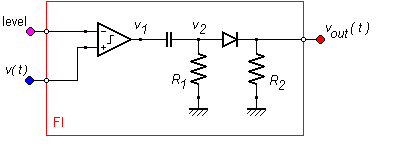
\includegraphics[scale = 1.5]{Frequenzimetro blocco.png}
\end{figure}

\newpage 

\section{Frequenzimetro}
\footnote{Slide della prof | SDME 4 Strumenti numerici indicatori - parte II | pag 2 \\  
Appunti | 2025-04-15 | pag 10 | 2025-04-23 | pag 7}

Un altro strumento molto importante impiegato nell'ambito delle misure è il frequenzimetro, 
che è quello strumento che misura la frequenza del segnale. \newline 

Abbiamo già visto strumenti che misurano il tempo, ma approfondiremo strumenti che prendono il nome di strumenti reciprocali. \newline 

Gli strumenti reciprocali sono quegli strumenti che sfruttano il legame tra tempo e frequenza e scelgono automaticamente 
se misurare nel tempo o in frequenza in base al segnale sotto misura. \newline 

Un esempio di frequenzimetro numerico: 

\begin{figure}[h]
    \centering
    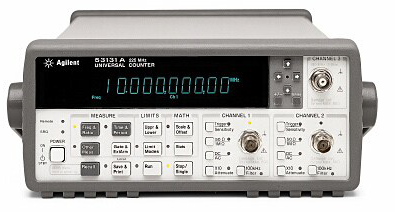
\includegraphics[scale = 1]{Frequenzimetro da banco.png}
\end{figure}

\newpage 

\section{Frequenzimetro e frequenza}
\footnote{Slide della prof | SDME 4 Strumenti numerici indicatori - parte II | pag 3 \\  
Appunti | 2025-04-15 | pag 10 | 2025-04-23 | pag 7}

Con il frequenzimetro si misura la frequenza f di un segnale elettronico analogico. \newline 

Sembra banale ripetere la definizione di frequenza, ma in realtà questa parola ha diverse definizioni in base al caso 
di cui si vuole studiare e osservare. \newline 

Per frequenza si intende la frequenza di un fenomeno ripetitivo, 
cioè il rapporto tra il numero degli eventi che si verificano in un arbitrario intervallo di tempo e la durata di tale intervallo. \newline 

La definizione sopra riportata non parla di eventi equi-spaziati o di segnale periodico. \newline 

Quindi, la frequenza dà un'informazione media, mediata sull'intervallo di tempo in cui abbiamo contato gli eventi. \newline 

Nel caso di un segnale periodico, 
i valori della frequenza e del periodo sono legati dal seguente vincolo: 

{
    \Large 
    \begin{equation}
        f = \frac{1}{T}
    \end{equation}
}

\newpage 

\section{Frequenzimetro - blocco FI}
\footnote{Slide della prof | SDME 4 Strumenti numerici indicatori - parte II | pag 4 - 6 \\  
Appunti | 2025-04-15 | pag 10 | 2025-04-23 | pag 8 | 2025-06-23 Ricevimento | pag 1, 5}

Di seguito lo schema a blocchi del frequenzimetro: 

\begin{figure}[h]
    \centering
    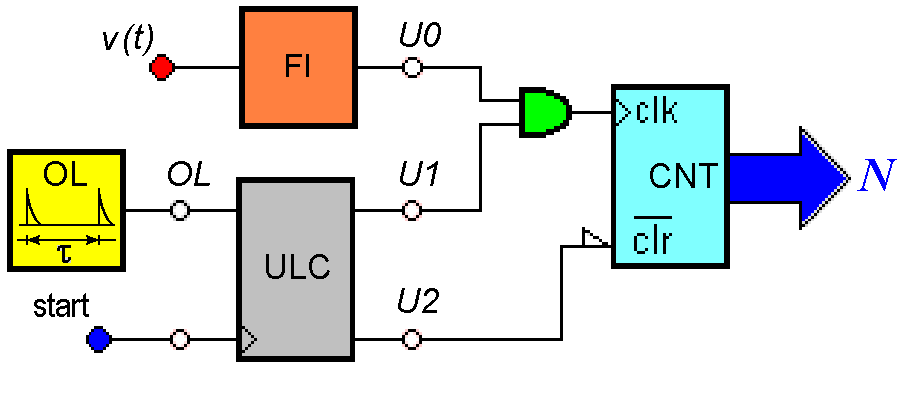
\includegraphics[scale = 0.8]{Frequenzimetro schema a blocchi.png}
\end{figure}

Tranne il blocco FI in arancione, 
i componenti sono gli stessi dell'intervallometro, 
ma la disposizione è diversa. \newline 

L'oscillatore locale OL è collegato come ingresso all'ULC, 
invece il blocco Formatore di Impulsi FI è collegato all'ingresso del gate, 
che è la porta logica AND. \newline 

Inoltre v(t), il segnale analogico da misurare, non va in ingresso all'ULC, 
bensì al blocco FI. \newline 

In un intervallometro e periodometro l'OL doveva avere un periodo $\tau$ molto breve rispetto al periodo da misurare: 
nell'intervallo di tempo si andranno a contare gli eventi che si sono verificati nel segnale v(t). \newline 

Di seguito un esploso del blocco FI: 

\begin{figure}[h]
    \centering
    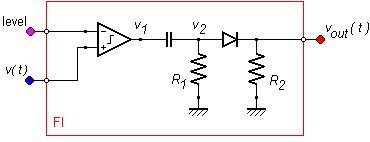
\includegraphics[scale = 1.2]{Blocco Formatore di impulsi FI esploso.png}
\end{figure}

La configurazione con condensatore e resistore (nella figura condensatore C e resistore $R_1$), osservando i componenti in frequenza, 
formano un filtro passa-alto. \newline 

\begin{tcolorbox}
Il motivo per cui questa configurazione tra condensatore e resistore è un filtro passa alto è approfondito in questo link: \\
\url{https://www.edutecnica.it/elettronica/filtrip/filtrip.htm}    
\end{tcolorbox}

La funzione del blocco "formatore di impulsi" FI è quella di generare un impulso positivo ad ogni occorrenza del segnale v(t). \newline 

Il principio di funzionamento del diodo è il seguente: 

\begin{figure}[h]
    \centering
    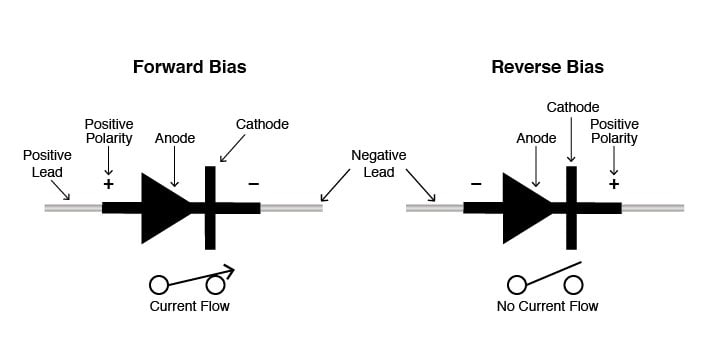
\includegraphics[scale = 0.5]{6004284b-dmm-how-to-diode-715x36.jpg}
\end{figure}

\newpage 

\begin{tcolorbox}
    Per approfondire cosa è un diodo e come funzione \\
    \url{https://www.fluke.com/it-it/informazioni/blog/tester/cose-un-diodo}
\end{tcolorbox}

La presenza del diodo nel blocco FI è molto importante perchè si escludono gli impulsi negativi, 
sennò si misurerebbero anche le transizioni basse del segnale. \newline 

Per transizioni basse si intende quando il segnale da un certo valore diminuisce di una certa soglia prefissata. \newline 

Supponiamo di avere in ingresso al pin v(t) una tensione sinusoidale a valore medio nullo: 

\begin{figure}[h]
    \centering
    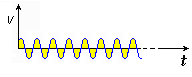
\includegraphics[scale = 2]{sinusoide a valore medio nullo.png}
\end{figure}

Impostiamo una soglia della tensione: 

\begin{figure}[h]
    \centering
    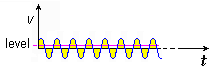
\includegraphics[scale = 2]{sinusoide a valore medio nullo con level.png}
\end{figure}

in figura è indicato come level. \newline 

In uscita al blocco comparatore (il triangolino in figura), cioè nel pin $v_1$, 
avremo che: 

\begin{itemize}
    \item se v(t) $>$ level, allora $v_1$ sarà alto 
    \item se v(t) $<$ level, allora $v_1$ sarà basso 
\end{itemize}

Troviamo che $v_1$ ha questo andamento: 

\begin{figure}[h]
    \centering
    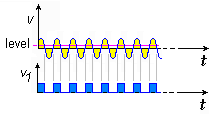
\includegraphics[scale = 2]{andamento del comparatore dato un segnale sinusoidale e un level.png}
\end{figure}

\newpage 

$v_1$ va in ingresso al filtro passa-alto (cioè la configurazione condensatore C e resistore $R_1$). \newline 

In uscita, cioè al pin $v_2$, del filtro avremo degli impulsi sia positivi che negativi. \newline 

Il segnale $v_2$ va in direzione del raddrizzatore a semi-onda (configurazione con diodo e resistore). \newline 

\begin{tcolorbox}
    Per approfondire cosa è un raddrizzatore a semi onda: \\
    \url{https://www.elemania.altervista.org/diodi/pn/pn5.html}
\end{tcolorbox}

Il raddrizzatore toglie tutto l'andamento di $v_2$ quando è minore di zero. \newline 

Possiamo visualizzare tutti i pin del blocco FI come: 

\begin{figure}[h]
    \centering
    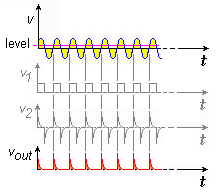
\includegraphics[scale = 2.5]{andamento dei segnale in un blocco FI.png}
\end{figure}

Per concludere, 
il blocco FI genera in uscita (cioè da v(t) a $v_{out}$) una successione di impulsi 
che presentano la stessa frequenza del segnale di ingresso. \newline 

\newpage

Una piccola osservazione riguardo agli andamenti reali del pin rispetto agli andamenti ideali: 

\begin{figure}[h]
    \centering
    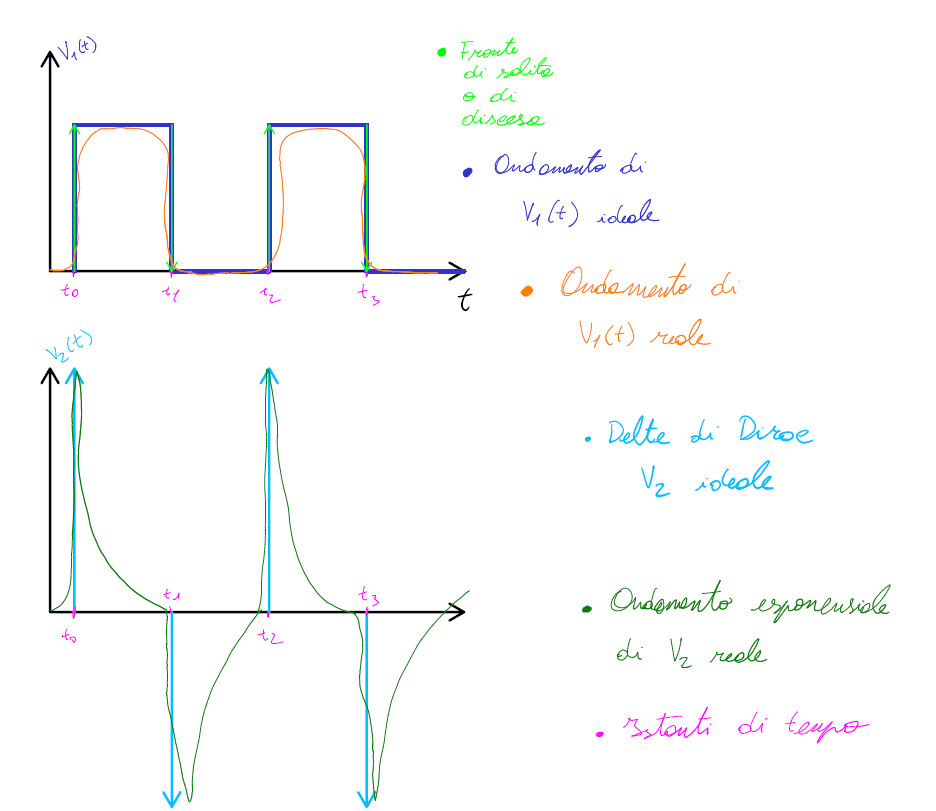
\includegraphics[scale = 0.8]{Andamenti delle tensioni in blocco FI del frequenzimetro.PNG}
\end{figure}

L'andamento reale di $v_1$ è quello di onde quadre con fronti d'onda ripidi: dal corso di Tds sappiamo che se si ha un fronte ripido nel tempo, in frequenza si avrà spettro infinito. \newline 

Avere spettro infinito, nella realtà non è possibile, quindi, $v_1$ avrà un andamento smussato nel tempo. \newline 

La coppia condensatore C e $R_1$ si comporta come derivatore, dalla legge caratteristica del condensatore. \newline 

La derivata di un fronte d'onda ripido, idealmente, è una Delta di Dirac. \newline 

Se c'è un fronte d'onda verso l'alto, si avrà una delta di Dirac positiva, 
se c'è un fronte d'onda verso il basso, si avrà una delta di Dirac negativa. \newline 

Ma nella realtà, si avrà un andamento esponenziale, che è un andamento molto veloce, che si avvicina nella realtà ad una Delta di Dirac. \newline 

Come studiato da Tds, se abbiamo una delta di Dirac in frequenza, dovremmo avere l'asse dei tempi che si estende per $[- \infty, + \infty]$ e ciò, nella realtà, non è possibile. \newline 

\newpage 

\section{Frequenzimetro numerico - schema di principio}
\footnote{Slide della prof | SDME 4 Strumenti numerici indicatori - parte II | pag 7 - 8 \\  
Appunti | 2025-04-23 | pag 8 - 9 | 2025-04-29 | pag 2}

Visto come funziona il blocco FI, vediamo quale è il funzionamento ideale di un frequenzimetro. \newline 

Dal seguente frequenzimetro: 

\begin{figure}[h]
    \centering
    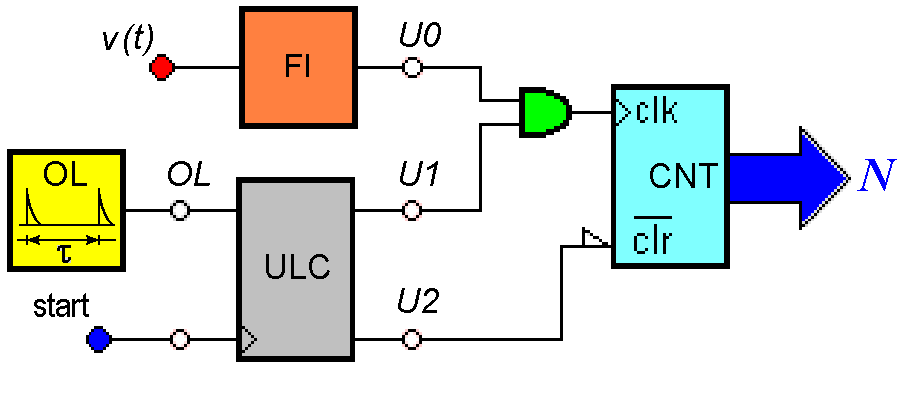
\includegraphics[scale = 0.8]{Frequenzimetro schema a blocchi.png}
\end{figure}

è possibile ricavare la frequenza del segnale con la seguente formula: 

{
    \Large 
    \begin{equation}
        f = \frac{N}{\tau}
    \end{equation}
}

dove N è il numero contato dal CNT e $\tau$ è il periodo dell'impulso dell'OL. \newline 

Da un punto di vista matematico, 
possiamo calcolarci l'incertezza di f facendo le derivate parziali di $\tau$ e N: 

{
    \Large 
    \begin{equation}
        \frac{\Delta f}{f}
        =
        \frac{\Delta N}{N}
        - 
        \frac{\Delta \tau}{\tau}
    \end{equation}
}

Matematicamente questa formula è corretta, 
MA, e questo è un grosso ma, la GUM ci dice che un contributo 
di incertezza non potrà mai essere negativo: 
bisogna sovrastimare piuttosto che sottostimare. \newline 

Quindi dalla formula di $\frac{\Delta f}{f}$: 

{
    \Large 
    \begin{equation}
        - 
        \frac{\Delta \tau}{\tau}
        \rightarrow
        + 
        \frac{\Delta \tau}{\tau}
    \end{equation}
}

Sapendo ciò, 
l'incertezza della frequenza data dal frequenzimetro sarà:

{
    \Large 
    \begin{equation}
        \frac{\Delta f}{f}
        =
        \frac{\Delta N}{N}
        + 
        \frac{\Delta \tau}{\tau}
    \end{equation}
}

$\frac{\Delta \tau}{\tau} $ dipende dalla bontà dell'oscillatore locale, 
che se l'oscillatore fa il suo dovere (cit. Francescangeli): 

{
    \Large 
    \begin{equation}
        \frac{\Delta \tau}{\tau} = 0
    \end{equation}
}

Inoltre, possiamo riscrivere la formula della frequenza f anche come: 

{
    \Large 
    \begin{equation}
        \begin{split}
            f &= \frac{N}{\tau}
            \\ 
            &\updownarrow
            \\ 
            N &= f \cdot \tau
        \end{split}
    \end{equation}
}

Questa "banale" formula, ci fa capire che la misurazione che andremo a svolgere sarà una misura media lungo il periodo $\tau$. \newline 

Se $\tau$ è un periodo molto lungo, non si riesce a capire se il segnale v(t) supera il level in tempi molto brevi. \newline
 

Visualizzando i grafici e lo schema è lo stesso principio di funzionamento dell'intervallometro: 

\begin{figure}[h]
    \centering
    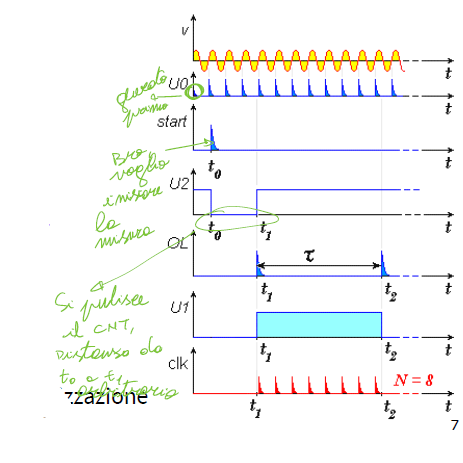
\includegraphics[scale = 1.5]{andamento dei segnali in un frequenzimetro.PNG}
\end{figure}

ma, in questo caso, l'ULC pone un segnale alto al primo fronte dell'OL (vedi a $t_1$ il pin U1) 
e poi ritorna basso al successivo fronte dell'OL (vedi U1 a $t_2$). \newline 

Come l'intervallometro, anche il frequenzimetro è affetto dai problemi di quantizzazione e sincronismo. \newline 

\newpage 

\subsection{Frequenzimetro numerico: la quantizzazione}
\footnote{Slide della prof | SDME 4 Strumenti numerici indicatori - parte II | pag 9 \\  
Appunti | 2025-04-15 | pag 9}

Consideriamo il caso classico di un frequenzimetro con i seguenti andamenti nei pin: 

\begin{figure}[h]
    \centering
    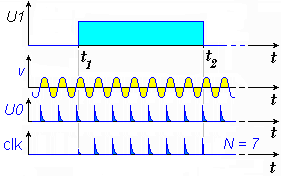
\includegraphics[scale = 1.5]{andamenti in un frequenzimetro con N = 7.png}
\end{figure}

in cui all'uscita N = 7. \newline 

Invece consideriamo un segnale analogico v(t) (v(t) in rosso) che ha una frequenza lievemente maggiore rispetto al caso precedente (v(t) in blu): 

\begin{figure}[h]
    \centering
    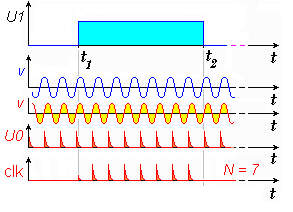
\includegraphics[scale = 1.5]{andamenti in un frequenzimetro con N = 7 con frequenza maggiore.png}
\end{figure}

Lo strumento non riesce a discriminare segnali che presentano differenze limitate nei loro valori di frequenza, 
perchè, come scritto nella sezione precedente, il frequenzimetro fa una media degli impulsi nel periodo $\tau$ \newline

\newpage 

\subsection{Incertezza da mancanza di sincronismo}
\footnote{Slide della prof | SDME 4 Strumenti numerici indicatori - parte II | pag 10 \\  
Appunti | 2025-04-15 | pag 9 | 2025-04-29 | pag 2}

Come il caso dell'intervallometro, il frequenzimetro è affetto da incertezza dovuto al sincronismo. \newline 

Ponendo questi due casi di esempio: 

\begin{figure}[h]
    \centering
    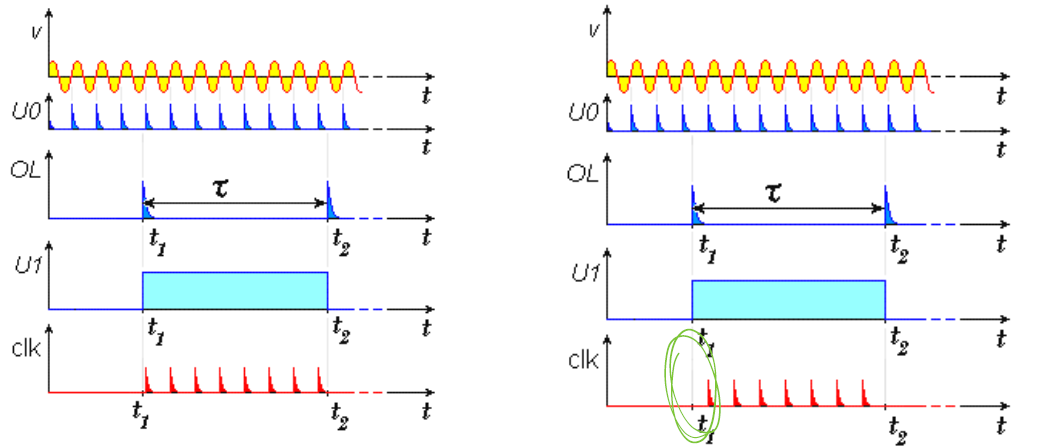
\includegraphics[scale = 0.8]{segnali del frequenzimetro dovuti al mancato sincronismo.PNG}
\end{figure}

Per mancanza di sincronismo, si è passato da N = 8 della figura a sinistra, 
a N = 7 della figura a destra. \newline 

Quindi, come il caso dell'intervallometro, l'incertezza $\Delta N$ è di: 

{
    \Large
    \begin{equation}
        \Delta N = \pm 1
    \end{equation}
}

L'incertezza è dovuta alla mancanza di sincronismo tra gli impulsi rilasciati dall'OL e quelli generati dal circuito FI: 
a seconda della fase del segnale dell'OL, il conteggio N cambia di $\pm 1$. \newline

\newpage 

\subsection{Incertezza complessiva}
\footnote{Slide della prof | SDME 4 Strumenti numerici indicatori - parte II | pag 11 \\  
Appunti | 2025-04-29 | pag 2}

Come il caso dell'intervallometro (vero lo sto scrivendo troppe volte, ma è vero, la formula ed i procedimenti sono gli stessi) 
l'incertezza della frequenza f è: 

{
    \Large 
    \begin{equation}
        \frac{\Delta f}{f}
        =
        \frac{\Delta N}{N}
        + 
        \frac{\Delta \tau}{\tau}
    \end{equation}
}

dove: 

\begin{itemize}
    \item $\frac{\Delta \tau}{\tau}$ dipende esclusivamente dalla qualità del campione di tempo utilizzato, cioè dal $\tau$ dell'OL 
    \item $\frac{\Delta N}{N}$ dipende dal prodotto fra frequenza del segnale sotto misurazione ed il prodotto dell'OL usato come campione di tempo
\end{itemize}

Si può trarre queste conclusioni per $\frac{\Delta N}{N}$ perchè: 

{
    \Large 
    \begin{equation}
        \begin{split}
            f &= \frac{N}{\tau}
            \\ 
            &\updownarrow
            \\ 
            N &= f \cdot \tau
        \end{split}
    \end{equation}
}

allora: 

{
    \Large 
    \begin{equation}
        \begin{cases}
        \Delta N = \pm 1 
        \\ 
        N = f \cdot \tau
        \\
        \frac{\Delta N}{N} = \pm \frac{1}{N} = \pm \frac{1}{(f \cdot \tau)}
    \end{cases}
    \end{equation}
}

Quindi, se vogliamo diminuire l'incertezza di N, cioè $\frac{\Delta N}{N}$ deve diminuire, 
allora il denominatore di $\frac{\Delta N}{N}$, cioè $(f \cdot \tau)$, deve essere il più elevato possibile. \newline 

Per fare ciò o si ha una frequenza del segnale f molto elevata, con $\tau$ dell'OL molto breve, 
oppure se si ha una frequenza f bassa, bisogna avere un $\tau$ dell'OL di periodo maggiore. \newline 

Questo ultimo caso ci esprime che maggiore è il dispendio di tempo per fare la misura, 
maggiore sarà il costo, 
ma, soprattutto, si rischia  
che la valutazione media fatta su un periodo troppo lungo non riesca a cogliere eventuali fluttuazioni della frequenza del segnale.\newline 

\newpage 

\section{Frequenzimetro: regolazione di level, slope e isteresi per minimizzare il rumore}
\footnote{Slide della prof | SDME 4 Strumenti numerici indicatori - parte II | pag 12 - 14 \\  
Appunti | 2025-04-29 | pag 3} 

Come il caso del periodometro, nel frequenzimetro è possibile regolare il valore di level e di slope del segnale di misura. \newline 

Il valore del "level" è la soglia per andare a pilotare la generazione degli impulsi: può essere regolato da un comando dello strumento. \newline 

Lo "slope", cioè la pendenza del segnale, può essere scelta o positiva o negativa, 
a seconda che vogliamo lavorare sul fronte di salita o di discesa di attraversamento del level. \newline 

Questa scelta va opportunamente fatta in base alle caratteristiche del segnale da esaminare. \newline 

\begin{tcolorbox}
    Per questo motivo, se possibile, è meglio visualizzare con un oscilloscopio il segnale, prima di svolgere la misura, e poi utilizzare il frequenzimetro e /o altri strumenti di misura
\end{tcolorbox}

Come il caso del periodometro, è opportuno scegliere il punto in cui il segnale presenta una variazione molto ripida. \newline 

Questa scelta riguardo alla pendenza non deve essere fatta per un problema di jitter, 
come era accaduto nel periodometro, 
bensì a causa delle false commutazioni. \newline 

Il problema del jitter rimane anche nel frequenzimetro reale, ma le false commutazioni sono un problema maggiore rispetto al jitter. \newline 

Per contrastare le false commutazioni, nel frequenzimetro può essere impostato e regolato l'isteresi. \newline 

In un frequenzimetro reale, l'isteresi e il level possono essere cambiati da una manopola dedicata: 

\begin{figure}[h]
    \centering
    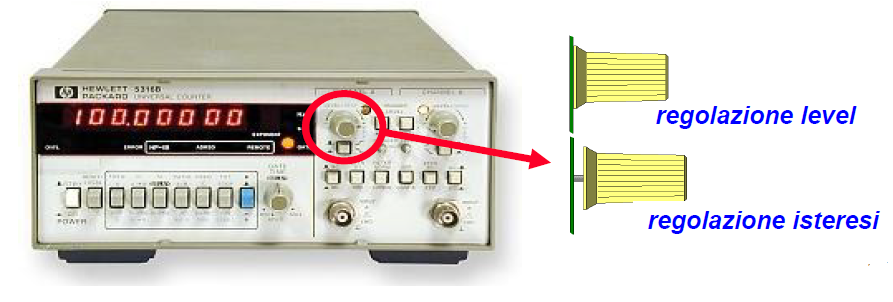
\includegraphics[scale = 0.5]{regolazione level e isteresi in un frequenzimetro reale.PNG}
\end{figure}

Come possiamo visualizzare dalla seguente schermata: 

\begin{figure}[h]
    \centering
    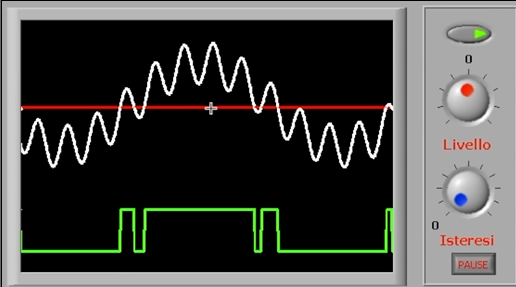
\includegraphics[scale = 0.8]{segnale sovrapposto a rumore con passaggio al level.png}
\end{figure}

dove il segnale bianco è il segnale utile (che consideriamo una sinusoide) sovrapposto a un rumore a una frequenza maggiore, 
la linea rossa è il level e il segnale verde indica se il segnale misurato ha avuto una transizione lungo il level fissato. \newline 

La presenza di rumore sovrapposto al segnale utile può comportare a delle transizioni spurie sul segnale che esce dal comparatore, 
perchè ci saranno attraversamenti della soglia "level" di quelli che effettivamente vogliamo rilevare. \newline 

Se applicassi questo segnale al filtro passa-alto e al raddrizzatore, 
il circuito FI genererebbe tre impulsi anziché uno per ogni ciclo del segnale utile 
e misurerei una frequenza 3 volte superiore di quella effettiva. \newline 

Invece applicando l'isteresi: 

\begin{figure}[h]
    \centering
    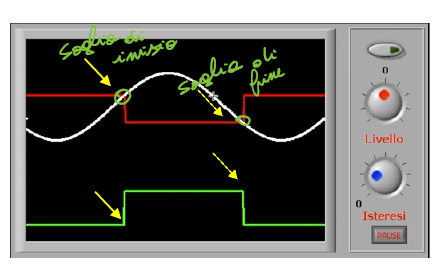
\includegraphics[scale = 1]{segnale con isteresi.png}
\end{figure}

piuttosto che applicare una soglia di level piatta si applicano 
due livelli di soglia differenti e si può risolvere il problema dovuto al rumore. \newline 

Impostando l'isteresi ad un segnale con rumore: 

\begin{figure}[h]
    \centering
    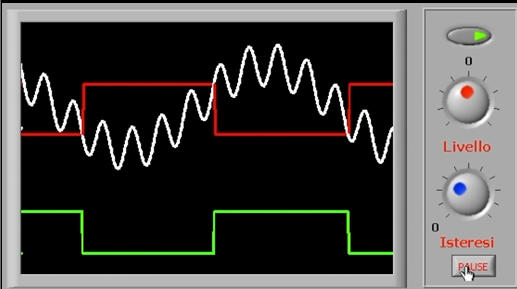
\includegraphics[scale = 0.8]{segnale con rumore con isteresi.png}
\end{figure}

permette di evitare i problemi citati dovuto al passaggio al "level". \newline 

Generalmente in elettronica si cerca di togliere l'isteresi perchè l'isteresi è dovuta ad un effetto di memoria, 
ad esempio di un condensatore, ma qui l'isteresi è voluta a causa del passaggio al level per il comparatore. \newline 

L'isteresi deve essere più ampia del valore picco-picco del rumore. \newline 

Se imposto una isteresi maggiore del valore picco-picco del segnale utile, la frequenza crolla a zero, non ci sono più impulsi che incrementano il contatore. \newline 

I valori di isteresi che permettono di ottenere una frequenza costante sono equivalenti, non ve ne è uno migliore, 
perchè tanto il segnale si ripete (se consideriamo solo un segnale periodico nel tempo). \newline 

I livelli vanno settati in corrispondenza dei punti di più rapida variazione del segnale utile. \newline 

Quindi, prima visualizziamo il segnale con rumore con un oscilloscopio, e poi impostiamo i valori di isteresi. \newline 

\newpage 

\section{Strumenti reciprocali}
\footnote{Slide della prof | SDME 4 Strumenti numerici indicatori - parte II | pag 15 - 18}

Gli strumenti reciprocali sono quegli strumenti che sfruttano il legame tra tempo e frequenza e scelgono automaticamente 
se misurare nel tempo o in frequenza in base al segnale sotto misura. \newline 

\subsection{Periodometro MPA (Multiple Period Averaging)}
\footnote{Slide della prof | SDME 4 Strumenti numerici indicatori - parte II | pag 15 - 18 \\  
Appunti | 2025-04-29 | pag 3 - 5}

Per strumenti MPA si intendono strumenti che svolgono la misura su multipli di un periodo e poi si svolge una media tra i valori. \newline 

Prendiamo per esempio il seguente caso. \newline 

Dato uno strumento che svolge solo una misura in un periodo: 

\begin{figure}[h]
    \centering
    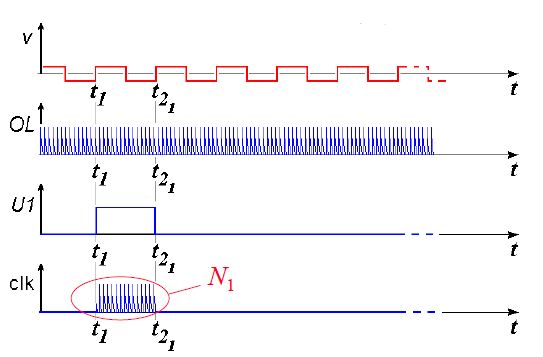
\includegraphics[scale = 0.7]{misura in un periodometro in un periodo.png}
\end{figure}


Come abbiamo precedentemente studiato, l'incertezza sul periodo T di N vale:

{
    \Large 
    \begin{equation}
        \begin{split}
            T &= N_1 \tau_1
            \\ 
            &\updownarrow
            \\
            \frac{\Delta N}{N}
            &= 
            \pm 
            \frac{1}{N_1}
        \end{split}
    \end{equation}
}

Se invece si considera una misura svolta su più periodi, cioè un approccio MPA: 

\begin{figure}[h]
    \centering
    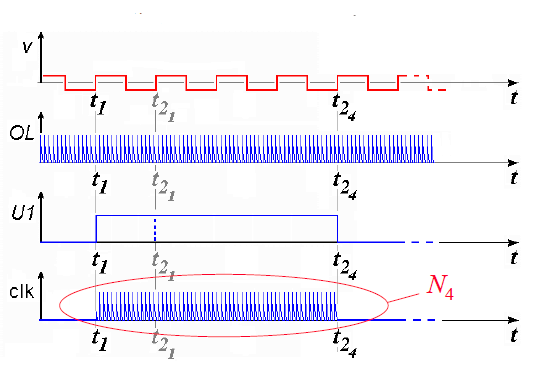
\includegraphics[scale = 0.8]{misura in un periodometro in multipli di un periodo.png}
\end{figure}

\newpage 

dove: 

{
    \Large 
    \begin{equation}
        N_4 = 4 N_1
    \end{equation}
}

allora l'incertezza della misura è: 

{
    \Large 
    \begin{equation}
        \begin{split}
            T = \frac{t_{24} - t_{21} }{4} &= \frac{N_4 \tau}{4}
            \\
            &\updownarrow
            \\
            \frac{\Delta N}{N} &= \pm \frac{1}{N_4} \simeq \pm \frac{1}{4 \cdot N_1}
        \end{split}
    \end{equation}
}

Si considera $\simeq \pm \frac{1}{4 \cdot N_1}$ per i problemi di sincronizzazione. \newline 

Come si è notato dal seguente esempio: 

{
    \Large
    \begin{equation}
        \pm \frac{1}{4 \cdot N_1} < \pm \frac{1}{N_1}
    \end{equation}
}

la misura svolta su multipli di un periodo T comporta una misura con incertezza minore. \newline 

L'approccio MPA può essere svolto solo se nei due periodi considerati il segnale è periodico, cioè si ripete. \newline 

Generalizzando l'approccio ad un multiplo qualsiasi di un periodo T, considerando k intero: 

{
    \Large 
    \begin{equation}
        \begin{split}
            T &= N_k \tau
            \\ 
            &\updownarrow
            \\
            \frac{\Delta N}{N}
            &= 
            \pm 
            \frac{1}{N_k}
            \simeq 
            \frac{1}{k \cdot N_1}
        \end{split}
    \end{equation}
}

Siccome si va a considerare un periodo più elevato (o in altri termini, considerando una finestra di misura più ampia) 
in generale, un periodometro MPA avrà bisogno di un registro più elevato rispetto ad uno strumento in cui si fa la misura solo in un unico periodo, cioè k = 1. \newline 

Il fattore k scelto sarà grande in modo proporzionale alla grandezza del registro e il periodo $\tau$ del clock. \newline 

\newpage 

\subsection{Incertezza relativa nella misura del periodo: confronto intervallometro convenzionale con strumento MPA}
\footnote{Slide della prof | SDME 4 Strumenti numerici indicatori - parte II | pag 19 - 20 \\  
Appunti | 2025-04-29 | pag 5} 

Come si può notare dalla seguente figura di esempio: 

\begin{figure}[h]
    \centering
    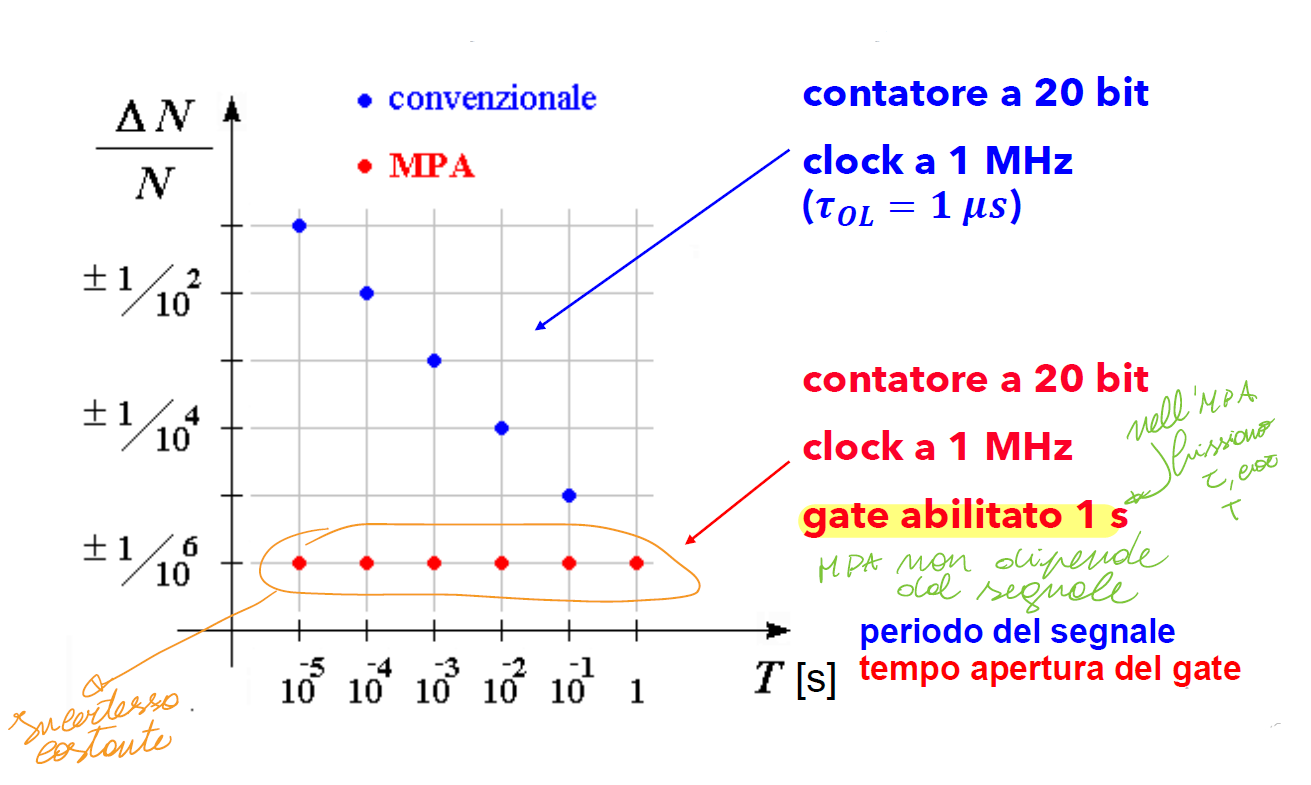
\includegraphics[scale = 0.4]{Confronto tra misura in un periodo e misura in periodi multipli.PNG}
\end{figure}

Il periodometro MPA non dipende dal periodo del segnale, bensì da quanto tempo è stato aperto il gate di misura: ecco perchè l'incertezza rimane costante. \newline 

\newpage 

\subsection{Frequenzimetro reciprocale}
\footnote{Slide della prof | SDME 4 Strumenti numerici indicatori - parte II | pag 21 - 22 \\  
Appunti | 2025-04-29 | pag 5 - 6}

Se il segnale è periodico, allora valgono i seguenti legami: 

{
    \Large 
    \begin{equation}
        \begin{cases}
            f = \frac{1}{T}
            \\ 
            \frac{\Delta f}{f} = \frac{\Delta T}{T}
        \end{cases}
    \end{equation}
}

Se il segnale ha una frequenza inferiore ad un valore critico, 
dipendente dalla frequenza del clock interno, 
lo strumento selezione automaticamente la misurazione di T e calcola analiticamente: 

{
    \Large 
    \begin{equation}
        f = \frac{1}{T}
    \end{equation}
}

con una incertezza relativa di conteggio che è indipendente da f. \newline 

\begin{figure}[h]
    \centering
    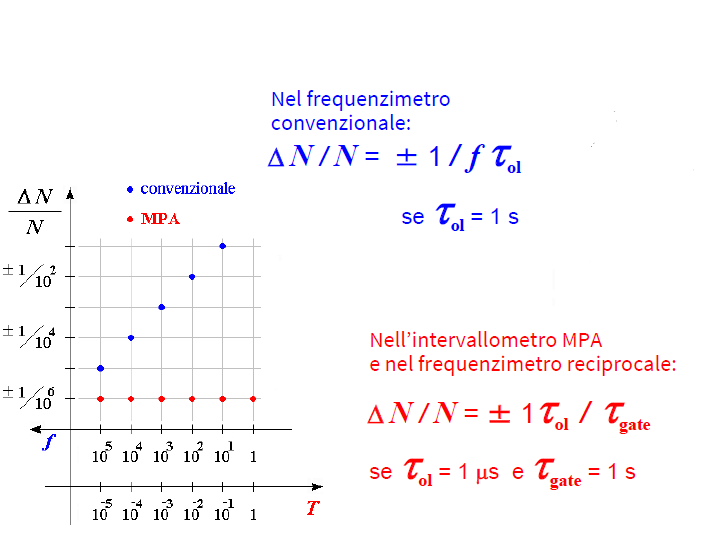
\includegraphics[scale = 0.8]{Confronto tra misura della frequenza svolta in un periodo contro quella in multipli di un periodo.png}
\end{figure}

Le stesse considerazioni svolte sul periodometro reciprocale MPA, 
le possiamo replicare sul frequenzimetro reciprocale. \newline 

\newpage